%%%%%%%%%%%%%%%%%%%%%%%%%%%%%%%%%%%%%%%%%
% Short Sectioned Assignment
% LaTeX Template
% Version 1.0 (5/5/12)
%
% This template has been downloaded from:
% http://www.LaTeXTemplates.com
%
% Original author:
% Frits Wenneker (http://www.howtotex.com)
%
% License:
% CC BY-NC-SA 3.0 (http://creativecommons.org/licenses/by-nc-sa/3.0/)
%
%%%%%%%%%%%%%%%%%%%%%%%%%%%%%%%%%%%%%%%%%

%----------------------------------------------------------------------------------------
%	PACKAGES AND OTHER DOCUMENT CONFIGURATIONS
%----------------------------------------------------------------------------------------

\documentclass[paper=a4, fontsize=11pt]{scrartcl} % A4 paper and 11pt font size

\usepackage[T1]{fontenc} % Use 8-bit encoding that has 256 glyphs
\usepackage{fourier} % Use the Adobe Utopia font for the document - comment this line to return to the LaTeX default
\usepackage[english]{babel} % English language/hyphenation
\usepackage{amsmath,amsfonts,amsthm} % Math packages
\usepackage[utf8]{inputenc} %For words with accents

\usepackage{lipsum} % Used for inserting dummy 'Lorem ipsum' text into the template

\usepackage{sectsty} % Allows customizing section commands

\usepackage{graphicx} % Required for including images
\graphicspath{{Figures/}} % Set the default folder for images
\usepackage[hidelinks]{hyperref}

\usepackage{listings} %code interpreter
\lstset{language=Prolog}
\lstset{numbers=left, numberstyle=\small}


\allsectionsfont{\centering \normalfont\scshape} % Make all sections centered, the default font and small caps

\usepackage{fancyhdr} % Custom headers and footers

\pagestyle{fancyplain} % Makes all pages in the document conform to the custom headers and footers
\fancyhead{} % No page header - if you want one, create it in the same way as the footers below
\fancyfoot[L]{} % Empty left footer
\fancyfoot[C]{} % Empty center footer
\fancyfoot[R]{\thepage} % Page numbering for right footer
\renewcommand{\headrulewidth}{0pt} % Remove header underlines
\renewcommand{\footrulewidth}{0pt} % Remove footer underlines
\setlength{\headheight}{13.6pt} % Customize the height of the header

\numberwithin{equation}{section} % Number equations within sections (i.e. 1.1, 1.2, 2.1, 2.2 instead of 1, 2, 3, 4)
\numberwithin{figure}{section} % Number figures within sections (i.e. 1.1, 1.2, 2.1, 2.2 instead of 1, 2, 3, 4)
\numberwithin{table}{section} % Number tables within sections (i.e. 1.1, 1.2, 2.1, 2.2 instead of 1, 2, 3, 4)

\setlength\parindent{0pt} % Removes all indentation from paragraphs - comment this line for an assignment with lots of text

%----------------------------------------------------------------------------------------
%	TITLE SECTION
%----------------------------------------------------------------------------------------

\newcommand{\horrule}[1]{\rule{\linewidth}{#1}} % Create horizontal rule command with 1 argument of height

\title{	
\normalfont \normalsize 
\textsc{Programação em Lógica} \\ [25pt] % Your university, school and/or department name(s)
\horrule{0.5pt} \\[0.4cm] % Thin top horizontal rule
\huge Eigenstate \\ % The assignment title
\horrule{2pt} \\[0.5cm] % Thick bottom horizontal rule
}

\author{
	Ricardo Jorge de Araújo Ferreira\\
	\normalsize\itshape up200305418\\
	\small Projecto no github: \url{https://github.com/ricardojaferreira/Eigenstate}
} % Your name
%

\date{\normalsize\today} % Today's date or a custom date

\begin{document}

\maketitle % Print the title

%----------------------------------------------------------------------------------------
%	História
%----------------------------------------------------------------------------------------

\section{História}

Eigenstate é um jogo de tabuleiro criado por Martin Grider \cite{GameGeek:2018}. É um jogo para dois jogadores com regras simples mas que cresce em complexidade à medida que o jogo avança. Este jogo ainda não está disponível no mercado, mas prêve-se a criação de um projecto no kickstarter para isso acontecer.

Eigenstate foi inspirado nos jogos The Duke \cite{TheDuke:2013} e Onitama \cite{Onitama:2014}. Durante o seu desenvolvimento o autor escreveu vários cenários de jogabilidade e condições de victória, tendo pensado até num cenário semelhante ao checkmate do Xadréz. Mas no final, durante uma apresentação do jogo, decidiu manter apenas duas regras básicas. O jogador na sua vez só tem que mover uma peça e colocar dois novos "pegs" para possibilitar movimentos numa nova jogada. Termina com a eliminação das peças adversárias, no entanto, a condição de vitória ainda pode ser alterada na versão final.

O nome Eigenstate vem de um termo da física quântica que se refere ao possível movimento de uma partícula \cite{Chesstris:2018}.

%----------------------------------------------------------------------------------------
%	Regras
%----------------------------------------------------------------------------------------

\section{Regras}

\subsection{Configuração}

O jogo joga-se num tabuleiro quadrado com 36 células (6x6). Cada jogador escolhe uma cor e coloca todas as peças dessa cor, 6 peças por jogador, no seu lado do tabuleiro.

Todas as peças começam com dois pegs, um no centro que representa a posição actual da peça e outro peg que permite a peça avançar uma casa.

\begin{figure}[tb]
	\centering
	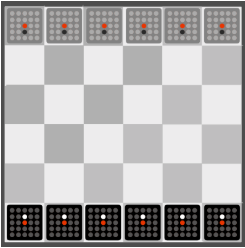
\includegraphics{eigenstate}
	\caption[Eigenstate Setup Inicial]{Eigenstate: Configuração inicial. \cite{eigenstaterules:2018}} % The text in the square bracket is the caption for the list of figures while the text in the curly brackets is the figure caption
	\label{fig:eigenstatestup} 
\end{figure}

\subsection{Jogabilidade}

Cada jogador no seu turno, se possível, deve:

\begin{enumerate}
	\item Mover uma das suas peças em conformidade com os pegs (como explicado mais à frente);
	\item Colocar dois pegs em qualquer uma das suas peças, na mesma, ou diferentes.
\end{enumerate}

O movimento das peças é regido pelo seguinte. Todos os pegs colocados na peça representam possíveis jogadas relativamente à sua posição actual. A posição actual é marcada pelo peg colocado no centro, tipicamente com uma cor diferente dos outros.

Este movimento está ilustrado na figura \ref{fig:eigenstatemoves}. Na figura é possível ver que o jogador moveu a peça 1 e colocou dois novos pegs, um na peça que moveu e outro na peça 2. Na próxima jogada, este jogador poderá mover a peça 1 para as posições a ou b e a peça 2 pode ser colocada nas posições d ou c. Estes movimentos correspondem à posição dos pegs em cada peça.

\begin{figure}[tb]
	\centering
	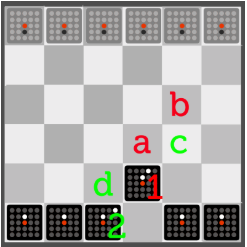
\includegraphics{eigenstate_moves}
	\caption[Eigenstate: Movimento das peças.]{Eigenstate: Movimento de peças. \cite{eigenstaterules:2018}} % The text in the square bracket is the caption for the list of figures while the text in the curly brackets is the figure caption
	\label{fig:eigenstatemoves} 
\end{figure}

O movimento das peças obdece ainda às seguintes regras:

\begin{itemize}
	\item Os pegs nunca podem ser removidos das peças, garantindo que as peças podem sempre avançar uma casa;
	\item As peças podem saltar por cima de outras peças;
	\item As peças não podem sair do tabuleiro;
	\item As peças não rodam;
	\item As peças só se podem mover para trás se tiverem pegs atrás do marcador central;
	\item Uma peça que se mova para a mesma posição de outra peça, faz com que a outra seja removida do tabuleiro;
	\item Peças do mesmo jogador, podem mover-se para cima uma das outras e as peças têm que ser removidas conforme a regra anterior.
\end{itemize}

A colocação de pegs, obdece às seguintes regras:

\begin{itemize}
	\item Só podem ser colocados em espaços livres, das peças do jogador não capturadas;
	\item Em cada turno podem ser colocados 2 pegs em peças diferentes ou na mesma;
	\item Não é necessário colocar nenhum peg na peça movida nessa ronda.
\end{itemize}

\subsection{Condição de Victória}

A forma principal de vitória consiste em reduzir o adversário a apenas uma peça. Num caso em que ambos os jogadores tenham duas peças cada um, a vitória pode ser conseguida se um jogador colocar pegs em todas as posições de uma das suas peças.


%----------------------------------------------------------------------------------------
%	Implementação em Prolog
%----------------------------------------------------------------------------------------

\section{Implementação em Prolog}

\subsection{Representação interna do estado do jogo}

Este jogo terá como representações principais o tabuleiro e a peça. Sendo que as peças são também elas tabuleiros para a colocação de pegs, a representação destes dois elementos será semelhante, embora a forma como se interpretam os resultados seja bastante diferente. Ambos terão uma representação baseada em listas de listas.

A representação inicial do tabuleiro será a seguinte:

\begin{lstlisting}
[
		['b1','b2','b3','b4','b5','b6'],
		['e','e','e','e','e','e'],
		['e','e','e','e','e','e'],
		['e','e','e','e','e','e'],
		['e','e','e','e','e','e'],
		['a1','a2','a3','a4','a5','a6']
]
\end{lstlisting}

O tabuleiro é uma lista com 6 sub-listas, uma para cada linha do tabuleiro. Com esta estrutura podemos pesquisar o tabuleiro de uma forma análoga a uma matriz, pesquisando por linha e coluna, tirando partido da divisão das listas em \emph{Head} e \emph{Tail}. Por exemplo, um predicado \emph{boardLine(X,L)} em que X é o número da linha e L o tabuleiro, pode ser utilizado de forma recursiva para percorrer na vertical. Um excerto de código para esta finalidade será:

\begin{lstlisting}
boardLine(_Z,[]).

boardLine(X,[H|T]):-
	Line is 1+X,
	boardColumn(C,H),
	boradLine(Line,T).
\end{lstlisting}

O predicado \emph{boardColumn(C,H)} terá uma função semelhante ao anterior mas irá percorrer a lista na horizontal, garantindo que são obtidos todos os elementos do tabuleiro. De notar que a recursividade apenas termina quando a lista fica vazia, significando que foram visitadas todas as células.

Tendo uma forma de pesquisar o tabuleiro, falta uma tradução do significado de cada átomo. Para isso podem ser utilizados predicados e estes adicionados à base de conhecimento do programa.  Estes predicados serão de particular interesse para a impressão do tabuleiro, uma vez que os átomos já têm valores bastante expressivos, ou seja,

\begin{itemize}
	\item 'e' -  célula vazia;
	\item 'aX' - célula com peça X do jogador 1;
	\item 'bX' - célula com peça X do jogador 2.
\end{itemize}

Como cada peça pode ter um estado diferente ao longo do jogo (dependendo do número de pegs que tem) é necessário uma representação individual de cada uma.

A aborgadem para a representação das peças será semelhante à tomada para o tabuleiro, embora com alguma complexidade acrescida. Cada peça será representada por uma lista com o seguinte formato (peça no estado inicial):

\begin{lstlisting}
[
	['o','o','o','o','o'],
	['o','o','*','o','o'],
	['o','o','@','o','o'],
	['o','o','o','o','o'],
	['o','o','o','o','o']
]
\end{lstlisting}

O método para percorrer as peças será o mesmo utilizado para o tabuleiro, pois cada peça, é ela própria um tabuleiro. Cada átomo nas peças terá o seguinte significado:

\begin{itemize}
	\item 'o' -  célula vazia, pode ser colocado um peg;
	\item '*' - célula com peg;
	\item '@' - célula central que marca a posição da peça no tabuleiro.
\end{itemize}

Uma peça num estado mais avançado do jogo poderá ter o seguinte estado:

\begin{lstlisting}
[
	['*','o','o','o','o'],
	['o','*','*','o','o'],
	['o','o','@','o','o'],
	['o','o','o','*','o'],
	['o','o','*','o','o']
]
\end{lstlisting}

O tabuleiro por sua vez poderá estar num estado semelhante ao seguinte:

\begin{lstlisting}
[
	['e','e','e','e','b5','b6'],
	['e','a5','e','e','b3','e'],
	['e','e','e','e','e','e'],
	['e','b2','e','e','e','e'],
	['e','e','e','e','e','e'],
	['a1','e','e','e','e','a6']
]
\end{lstlisting}

Num caso de victória por eliminação das peças do adversário, o tabuleiro estará num estado semelhante ao seguinte:

\begin{lstlisting}
[
	['e','e','e','e','b5','b6'],
	['e','e','e','e','b3','e'],
	['e','e','e','e','a3','e'],
	['e','b2','e','e','e','e'],
	['e','e','e','e','e','e'],
	['e','e','e','e','e','e']
]
\end{lstlisting}

Neste caso, o jogador 2 terá a victória pois o jogador 1 apenas tem a peça a3.

Num cenário em que cada jogador fica reduzido a apenas 2 peças cada, vence o jogador que conseguir colocar uma das suas peças no seguinte estado.

\begin{lstlisting}
[
	['*','*','*','*','*'],
	['*','*','*','*','*'],
	['*','*','@','*','*'],
	['*','*','*','*','*'],
	['*','*','*','*','*']
]
\end{lstlisting}


Na próxima secção serão apresentadas algumas imagens dos estados do tabuleiro durante o jogo.

\subsection{Visualização do tabuleiro em modo de texto}

O jogo está pensado para correr na consola e como tal terá uma representação com carácteres ASCII. Para a representação funcionar correctamente, recomenda-se uma consola com font do tipo monospace, para todos os carácteres ocuparem o mesmo espaço. As peças são representadas pelos mesmos simbolos utilizados na representação interna do jogo, as células do tabuleiro vazias utilizam um predicado de tradução que se baseia no facto da posição da célula ser par ou impar, para assim se conseguir uma distinçao entre células contíguas. Os predicados são:

\begin{lstlisting}
boardCell(1,'e',': : : : : : :').
boardCell(0,'e','             ').
\end{lstlisting}

o valor 0 ou 1 é conseguido através da avaliação do resto da divisição inteira por 2 do número da célula.

Uma representação inicial do tabuleiro pode ser vista na Figura \ref{fig:initstate}. O Jogador 1 tem as peças verdes e o jogador 2 as peças vermelhas.

O tabuleiro numa fase de jogo intermédia pode ser vista na Figura \ref{fig:middlestate} e na fase final na Figura \ref{fig:finalstate}.

\begin{figure}[tb]
	\centering
	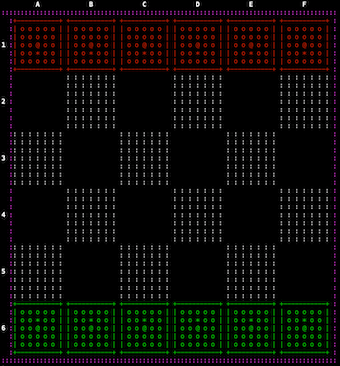
\includegraphics{tabuleiro_init}
	\caption[PROLOG: tabuleiro estado inicial]{Tabuleiro estado inicial} % The text in the square bracket is the caption for the list of figures while the text in the curly brackets is the figure caption
	\label{fig:initstate} 
\end{figure}

\begin{figure}[tb]
	\centering
	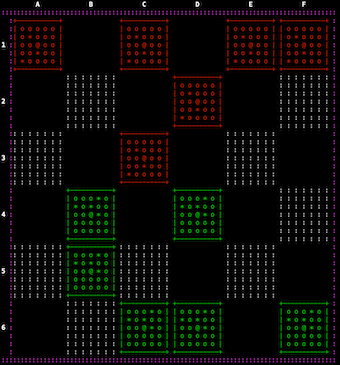
\includegraphics{tabuleiro_middle}
	\caption[PROLOG: tabuleiro estado intermédio]{Tabuleiro estado intermédio} % The text in the square bracket is the caption for the list of figures while the text in the curly brackets is the figure caption
	\label{fig:middlestate} 
\end{figure}

\begin{figure}[tb]
	\centering
	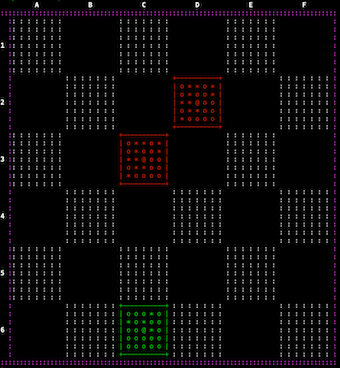
\includegraphics{tabuleiro_final}
	\caption[PROLOG: tabuleiro estado final]{Tabuleiro estado final} % The text in the square bracket is the caption for the list of figures while the text in the curly brackets is the figure caption
	\label{fig:finalstate} 
\end{figure}

%----------------------------------------------------------------------------------------
%	BIBLIOGRAPHY
%----------------------------------------------------------------------------------------
\renewcommand{\refname}{\spacedlowsmallcaps{Referências}} 
\bibliographystyle{unsrturl}
\bibliography{sample.bib}


\end{document}